\batchmode
\documentclass{beamer}
\usepackage[utf8]{inputenc}
\usepackage[ngerman]{babel}
\usepackage{amsmath}

\usetheme[deutsch]{KIT}
\author{Jan Haag (jan.haag@student.kit.edu)}
\title{Programmieren Tutorium 9 -- Rekursion}
\institute{Institut f\"{u}r Zeritfizierbare und Vertrauensw\"{u}rdige Informatiksysteme (ZVI)}
\TitleImage[scale=0.225]{frontpic.jpg}

\begin{document}
\begin{frame}
\maketitle
\end{frame}

\begin{frame}
\frametitle{Inhalt}
\tableofcontents
\end{frame}

\section{Rekursion}
\begin{frame}
\frametitle{Rekursion}

\includegraphics[scale=0.5]{rekursion.pdf}
\end{frame}

\section{Aufgaben}
\begin{frame}
\frametitle{Aufgabe 1}
Was tut das folgende Programm?
\end{frame}

\begin{frame}[shrink=15]
\setlength{\parindent}{0em}
\newcommand{\stylea}[1]{\noindent{\textcolor[rgb]{0.0, 0.0, 0.0}{\fcolorbox[rgb]{0, 0, 0}{1.0, 1.0, 1.0}{#1}}}}
\newcommand{\stylee}[1]{\noindent{\textcolor[rgb]{0.0, 0.5, 0.0}{\fcolorbox[rgb]{0, 0, 0}{1.0, 1.0, 1.0}{#1}}}}
\newcommand{\stylef}[1]{\noindent{\textbf{\textcolor[rgb]{0.0, 0.0, 0.5}{\fcolorbox[rgb]{0, 0, 0}{1.0, 1.0, 1.0}{#1}}}}}
\newcommand{\styleg}[1]{\noindent{\textcolor[rgb]{1.0, 0.6, 0.1}{\fcolorbox[rgb]{0, 0, 0}{1.0, 1.0, 1.0}{#1}}}}
\newcommand{\stylek}[1]{\noindent{\textcolor[rgb]{0.2, 0.1, 0.1}{\fcolorbox[rgb]{0, 0, 0}{1.0, 1.0, 1.0}{#1}}}}
\newcommand{\stylel}[1]{\noindent{\textcolor[rgb]{0.0, 0.0, 0.0}{\fcolorbox[rgb]{0, 0, 0}{1.0, 1.0, 1.0}{#1}}}}
\newcommand{\styleq}[1]{\noindent{\textbf{\textcolor[rgb]{0.6, 0.1, 0.1}{\fcolorbox[rgb]{0, 0, 0}{1.0, 1.0, 1.0}{#1}}}}}
\newcommand{\stylet}[1]{\noindent{\textbf{\textcolor[rgb]{0.0, 0.0, 0.8}{\fcolorbox[rgb]{0, 0, 0}{1.0, 1.0, 1.0}{#1}}}}}

\ttfamily
\setlength{\fboxrule}{0pt}
\setlength{\fboxsep}{0pt}
\stylea{{\hspace*{1em}}{\hspace*{1em}}}
\stylef{public}
\stylef{static}
\styleq{void}
\stylel{main}\stylek{(}\styleq{int}
\stylel{n}\stylek{)}
\stylek{\{}
\stylea{} \\
\stylea{{\hspace*{1em}}{\hspace*{1em}}{\hspace*{1em}}{\hspace*{1em}}}
\stylel{\_}\stylek{(}\stylee{1}\stylek{,}
\stylel{n}\stylek{,}
\stylel{n}\stylek{);}
\stylea{} \\
\stylea{{\hspace*{1em}}{\hspace*{1em}}}
\stylek{\}}
\stylea{} \\
\stylea{{\hspace*{1em}}{\hspace*{1em}}}
\stylef{private}
\stylef{static}
\styleq{void}
\stylel{\_}\stylek{(}\styleq{int}
\stylel{n}\stylek{,}
\styleq{int}
\stylel{x}\stylek{,}
\styleq{int}
\stylel{y}\stylek{)}
\stylek{\{}
\stylea{} \\
\stylea{{\hspace*{1em}}{\hspace*{1em}}{\hspace*{1em}}{\hspace*{1em}}}
\stylef{if}
\stylek{(}\stylel{x}
\stylek{<=}
\stylee{0}\stylek{)}
\stylel{t}\stylek{(}\stylel{y}\stylek{);}
\stylef{else}
\stylel{b}\stylek{(}\stylel{n}\stylek{,}
\stylel{x}\stylek{,}
\stylel{y}\stylek{);}
\stylea{} \\
\stylea{{\hspace*{1em}}{\hspace*{1em}}}
\stylek{\}}
\stylea{} \\
\stylea{{\hspace*{1em}}{\hspace*{1em}}}
\stylef{private}
\stylef{static}
\styleq{void}
\stylel{s}\stylek{(}\styleq{int}
\stylel{n}\stylek{)}
\stylek{\{}
\stylea{} \\
\stylea{{\hspace*{1em}}{\hspace*{1em}}{\hspace*{1em}}{\hspace*{1em}}}
\stylef{if}
\stylek{(}\stylel{n}
\stylek{<=}
\stylee{0}\stylek{)}
\stylef{return}\stylek{;}
\stylel{p}\stylek{(}\stylee{32}\stylek{);}
\stylel{s}\stylek{(}\stylel{n}
\stylek{-}
\stylee{1}\stylek{);}
\stylea{} \\
\stylea{{\hspace*{1em}}{\hspace*{1em}}}
\stylek{\}}
\stylea{} \\
\stylea{{\hspace*{1em}}{\hspace*{1em}}}
\stylef{private}
\stylef{static}
\styleq{void}
\stylel{a}\stylek{(}\styleq{int}
\stylel{n}\stylek{)}
\stylek{\{}
\stylea{} \\
\stylea{{\hspace*{1em}}{\hspace*{1em}}{\hspace*{1em}}{\hspace*{1em}}}
\stylef{if}
\stylek{(}\stylel{n}
\stylek{<=}
\stylee{0}\stylek{)}
\stylef{return}\stylek{;}
\stylel{p}\stylek{(}\stylee{42}\stylek{);}
\stylel{a}\stylek{(}\stylel{n}
\stylek{-}
\stylee{1}\stylek{);}
\stylea{} \\
\stylea{{\hspace*{1em}}{\hspace*{1em}}}
\stylek{\}}
\stylea{} \\
\stylea{{\hspace*{1em}}{\hspace*{1em}}}
\stylef{private}
\stylef{static}
\styleq{void}
\stylel{t}\stylek{(}\styleq{int}
\stylel{n}\stylek{)}
\stylek{\{} \\
\stylea{{\hspace*{1em}}{\hspace*{1em}}{\hspace*{1em}}{\hspace*{1em}}}
\stylef{if}
\stylek{(}\stylel{n}
\stylek{<=}
\stylee{0}\stylek{)}
\stylef{return}\stylek{;}
\stylel{s}\stylek{(}\stylel{n}\stylek{);}
\stylel{p}\stylek{(}\stylee{124}\stylek{);}
\stylel{p}\stylek{(}\stylee{10}\stylek{);}
\stylea{} \\
\stylea{{\hspace*{1em}}{\hspace*{1em}}}
\stylek{\}}
\stylea{} \\
\stylea{{\hspace*{1em}}{\hspace*{1em}}}
\stylef{private}
\stylef{static}
\styleq{void}
\stylel{b}\stylek{(}\styleq{int}
\stylel{n}\stylek{,}
\styleq{int}
\stylel{x}\stylek{,}
\styleq{int}
\stylel{y}\stylek{)}
\stylek{\{}
\stylea{} \\
\stylea{{\hspace*{1em}}{\hspace*{1em}}{\hspace*{1em}}{\hspace*{1em}}}
\stylel{s}\stylek{(}\stylel{x}\stylek{);}
\stylel{a}\stylek{(}\stylel{n}\stylek{);}
\stylel{p}\stylek{(}\stylee{10}\stylek{);}
\stylel{\_}\stylek{(}\stylel{n}
\stylek{+}
\stylee{2}\stylek{,}
\stylel{x}
\stylek{-}
\stylee{1}\stylek{,}
\stylel{y}\stylek{);}
\stylea{} \\
\stylea{{\hspace*{1em}}{\hspace*{1em}}}
\stylek{\}}
\stylea{} \\
\stylea{{\hspace*{1em}}{\hspace*{1em}}}
\stylef{private}
\stylef{static}
\styleq{void}
\stylel{p}\stylek{(}\styleq{int}
\stylel{c}\stylek{)}
\stylek{\{}
\stylea{} \\
\stylea{{\hspace*{1em}}{\hspace*{1em}}{\hspace*{1em}}{\hspace*{1em}}}
\stylel{System}\stylek{.}\stylel{out}\stylek{.}\stylel{print}\stylek{((}\styleq{char}\stylek{)}
\stylel{c}\stylek{);}
\stylea{} \\
\stylea{{\hspace*{1em}}{\hspace*{1em}}}
\stylek{\}}

\end{frame}

\begin{frame}[fragile]
\frametitle{Aufgabe}
Implementieren Sie einen L\"{o}sungsalgorithmus f\"{u}r die
T\"{u}rme von Hanoi.\\
Einf\"{u}hrung: \verb|http://goo.gl/1QYeh|\\
Musterl\"{o}sung: \verb|http://goo.gl/k8i7Z|\\
\end{frame}

\begin{frame}
\frametitle{Ende}
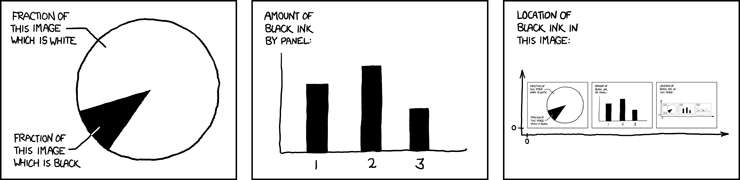
\includegraphics[scale=0.4]{self_description.png}
\end{frame}
\end{document}
